\chapter{Modelo Entidad-Relación}

\section{Reglas semánticas}

A continuación se describen las entidades que conforman el modelo, detallando los atributos que las caracterizan y las restricciones semánticas que las gobiernan. Las entidades se agrupan por módulo funcional para facilitar su comprensión.

\vspace{0.5cm}
\noindent \textbf{Módulo 1 Jerarquía de Personas}

\begin{itemize}
	\item \textbf{Persona} es la entidad abstracta base de toda persona registrada en el sistema. Toda persona es identificada de forma única por su DNI (clave alternativa de negocio) y por un ID\_Persona surrogado interno. Posee Nombres y Apellidos obligatorios, así como un Teléfono de contacto. El campo Email actúa como segunda clave única del sistema.
	\item \textbf{Cliente} es una subclase de Persona que representa al titular legal y financiero de la clínica: es quien registra mascotas a su nombre, firma autorizaciones y recibe las facturas. Extiende a Persona con una Dirección\_Principal obligatoria y un Contacto\_Emergencia opcional.
	\item \textbf{Empleado} es una subclase de Persona que representa a la fuerza laboral. Todo empleado posee un Código\_Empleado único interno, una Fecha\_Contratación y un Salario registrado como referencia administrativa.
	\item \textbf{Veterinario} es una subclase de Empleado que agrupa al personal médico habilitado para realizar actos clínicos con validez legal. Está identificado adicionalmente por su número de colegiatura CMPV (clave única) y declara una Especialidad médica.
	\item \textbf{Personal\_Apoyo} es una subclase de Empleado que representa al personal operativo no médico (recepcionistas, groomers, choferes). Posee un atributo Rol obligatorio que define su función dentro de la clínica, y un campo Licencia\_Conducir opcional, habilitado para el perfil de chofer.
\end{itemize}

\vspace{0.5cm}
\noindent \textbf{Módulo 2 Pacientes (Core Biológico)}

\begin{itemize}
	\item \textbf{Especie} representa el nivel más alto de clasificación biológica en el sistema (por ejemplo: Canino, Felino, Exótico). Está identificada por un ID\_Especie surrogado y su Nombre\_Especie es único e irrepetible.
	\item \textbf{Raza} representa la clasificación biológica específica de un animal. Está identificada por un ID\_Raza y un Nombre\_Raza. Toda raza pertenece obligatoriamente a una única Especie, lo que permite la trazabilidad biológica completa del paciente.
	\item \textbf{Mascota} es el perfil central del paciente. Posee un Nombre, una Fecha\_Nacimiento opcional, y un Sexo declarado de forma obligatoria. Toda mascota pertenece a una única Raza y está registrada bajo la responsabilidad de un único Cliente dueño.
	\item \textbf{Historial\_Médico} es el contenedor clínico permanente de la mascota. Toda mascota tiene exactamente un historial (relación 1:1 garantizada mediante una restricción UNIQUE sobre ID\_Mascota). Registra la Fecha\_Creación del expediente, el Grupo\_Sanguíneo y las Alergias\_Conocidas del paciente, ambas opcionales pero de alto valor clínico.
\end{itemize}

\vspace{0.5cm}
\noindent \textbf{Módulo 3 Catálogos e Inventario Especializado}

\begin{itemize}
	\item \textbf{Item\_Catálogo} es la superclase abstracta que unifica todo aquello que tiene un precio en la clínica, permitiendo facturación polimórfica. Posee un Nombre, un Precio Base obligatorio y un Tipo\_Item que discrimina si se trata de un servicio, un artículo de petshop o un medicamento.
	\item \textbf{Servicio} es una subclase de Item\_Catálogo que representa actividades intangibles ofrecidas por la clínica (consultas, cirugías, ecografías, baños). Indica mediante el atributo Requiere\_Veterinario si el servicio debe ser ejecutado por personal médico, y registra un Tiempo\_Estimado\_Min opcional para la gestión de agenda.
	\item \textbf{Artículo\_Petshop} es una subclase de Item\_Catálogo que representa los bienes físicos de la tienda (alimentos, accesorios, juguetes). Posee una Marca opcional, una Categoría obligatoria y un Stock\_General que controla el inventario de estos productos de forma global (no por lote), dado que no tienen fecha de caducidad crítica.
	\item \textbf{Medicamento} es una subclase de Item\_Catálogo que estandariza el vademécum de la clínica. Define el Principio\_Activo, la Concentración y la Presentación del fármaco, así como un indicador booleano Requiere\_Receta que condiciona su dispensación.
	\item \textbf{Lote\_Inventario} representa la existencia física de un medicamento en la farmacia. Un mismo medicamento puede tener múltiples lotes activos. Cada lote tiene una Fecha\_Caducidad, una Cantidad\_Inicial y un Stock\_Actual que se decrementa con cada dispensación o uso clínico registrado.
\end{itemize}

\vspace{0.5cm}
\noindent \textbf{Módulo 4 Flujo Médico (Corazón Clínico)}

\begin{itemize}
	\item \textbf{Cita} es la reserva de tiempo que organiza la agenda de la clínica. Vincula obligatoriamente a un Cliente solicitante, una Mascota paciente y un Empleado asignado. Registra la Fecha, la Hora, el Motivo de la visita y el Estado actual de la cita (pendiente, confirmada, completada, cancelada).
	\item \textbf{Atención\_Clínica} es el registro formal del acto médico asociado. Vincula la atención al Historial\_Médico del paciente y al Empleado (veterinario) responsable. Captura los signos vitales del triaje: Peso\_Kg, Temp\_C y Frecuencia\_Cardíaca, junto con la Anamnesis inicial. Fecha y hora son obligatorias para validez legal del acto.
	\item \textbf{Enfermedad\_Diagnóstico} es el catálogo de patologías estandarizado según la clasificación CIE. Cada enfermedad tiene un Código\_CIE único y un Nombre\_Enfermedad, lo que garantiza uniformidad en los registros médicos y permite reportes epidemiológicos precisos.
	\item \textbf{Resultado\_Diagnóstico} vincula una Atención Clínica con una Enfermedad\_Diagnóstico detectada. Clasifica el hallazgo mediante el atributo Tipo (presuntivo o definitivo) y puede incluir Observaciones adicionales del médico.
	\item \textbf{Procedimiento\_Aplicado} registra cada intervención médica ejecutada durante una atención (limpieza dental, cirugía, rayos X, etc.). Vincula la atención con el ítem de servicio del catálogo y almacena las Resultados\_Notas específicas de esa intervención.
	\item \textbf{Insumo\_Utilizado} es el descargador de inventario clínico. Registra qué Lote\_Inventario específico fue consumido durante una atención y en qué Cantidad\_Usada, permitiendo descontar el stock directamente del lote correcto al momento del acto médico.
	\item \textbf{Receta\_Médica} es la prescripción farmacológica emitida al dueño de la mascota. Vincula la atención con un Medicamento genérico (no con un lote), e indica la Dosis\_Frecuencia y la Duración\_Días del tratamiento a seguir en casa.
\end{itemize}

\vspace{0.5cm}
\noindent \textbf{Módulo 5 Operativo Anexo (Servicios de Valor Agregado)}

\begin{itemize}
	\item \textbf{Registro\_Estancia} controla la ocupación de las instalaciones de hospedaje e internamiento. Registra el Tipo de estadía (guardería vacacional o internamiento médico), la Fecha\_Ingreso, la Fecha\_Salida (opcional, hasta el momento del alta), el Nro\_Jaula asignado y las Instrucciones\_Cuidado pertinentes. Toda estancia está vinculada a una única Mascota.
	\item \textbf{Transporte\_Logística} gestiona el servicio de taxi veterinario de la clínica. Está vinculado a una Cita específica y a un Empleado con rol de chofer. Registra el Tipo\_Ruta (recojo o entrega), la Dirección\_Destino del servicio y el Estado actual del transporte (Pendiente, En curso, Completado, Cancelado).
\end{itemize}

\vspace{0.5cm}
\noindent \textbf{Módulo 6 Facturación y Finanzas}

\begin{itemize}
	\item \textbf{Factura} es el comprobante legal de la transacción económica. Registra la Fecha\_Emisión, el Subtotal, el IGV calculado y el Total a pagar. Está vinculada a un Cliente y, de forma opcional y mutuamente excluyente, a una Atención Clínica o a una Cita. Si ambas referencias son nulas, corresponde a una compra libre en el mostrador de petshop.
	\item \textbf{Detalle\_Factura} desglosa los ítems cobrados dentro de una factura. Por cada línea se registra el Item\_Catálogo facturado, la Cantidad, el Precio\_Unitario vigente y el Subtotal\_Línea. Si el ítem es un medicamento, el detalle vincula además el Lote\_Inventario específico despachado; si es una estancia, vincula el Registro\_Estancia correspondiente.
	\item \textbf{Pago} registra cada ingreso monetario recibido a cuenta de una factura. Permite que una misma factura sea abonada en múltiples cuotas o mediante diferentes medios. Por cada pago se registra la Fecha\_Pago, el Monto\_Abonado y el Método\_Pago utilizado (efectivo, tarjeta, Yape/Plin u otro).
\end{itemize}

\section{Modelo Entidad-Relación}

La figura 2.1 presenta el diagrama Entidad-Relación del sistema de base de datos de SOS Veterinaria, modelado bajo la notación de Pata de Gallo (Crow's Foot). El diagrama refleja la estructura completa de las 19 entidades descritas en la sección anterior, sus atributos, cardinalidades y restricciones de participación.

\begin{figure}[H]
	\centering
	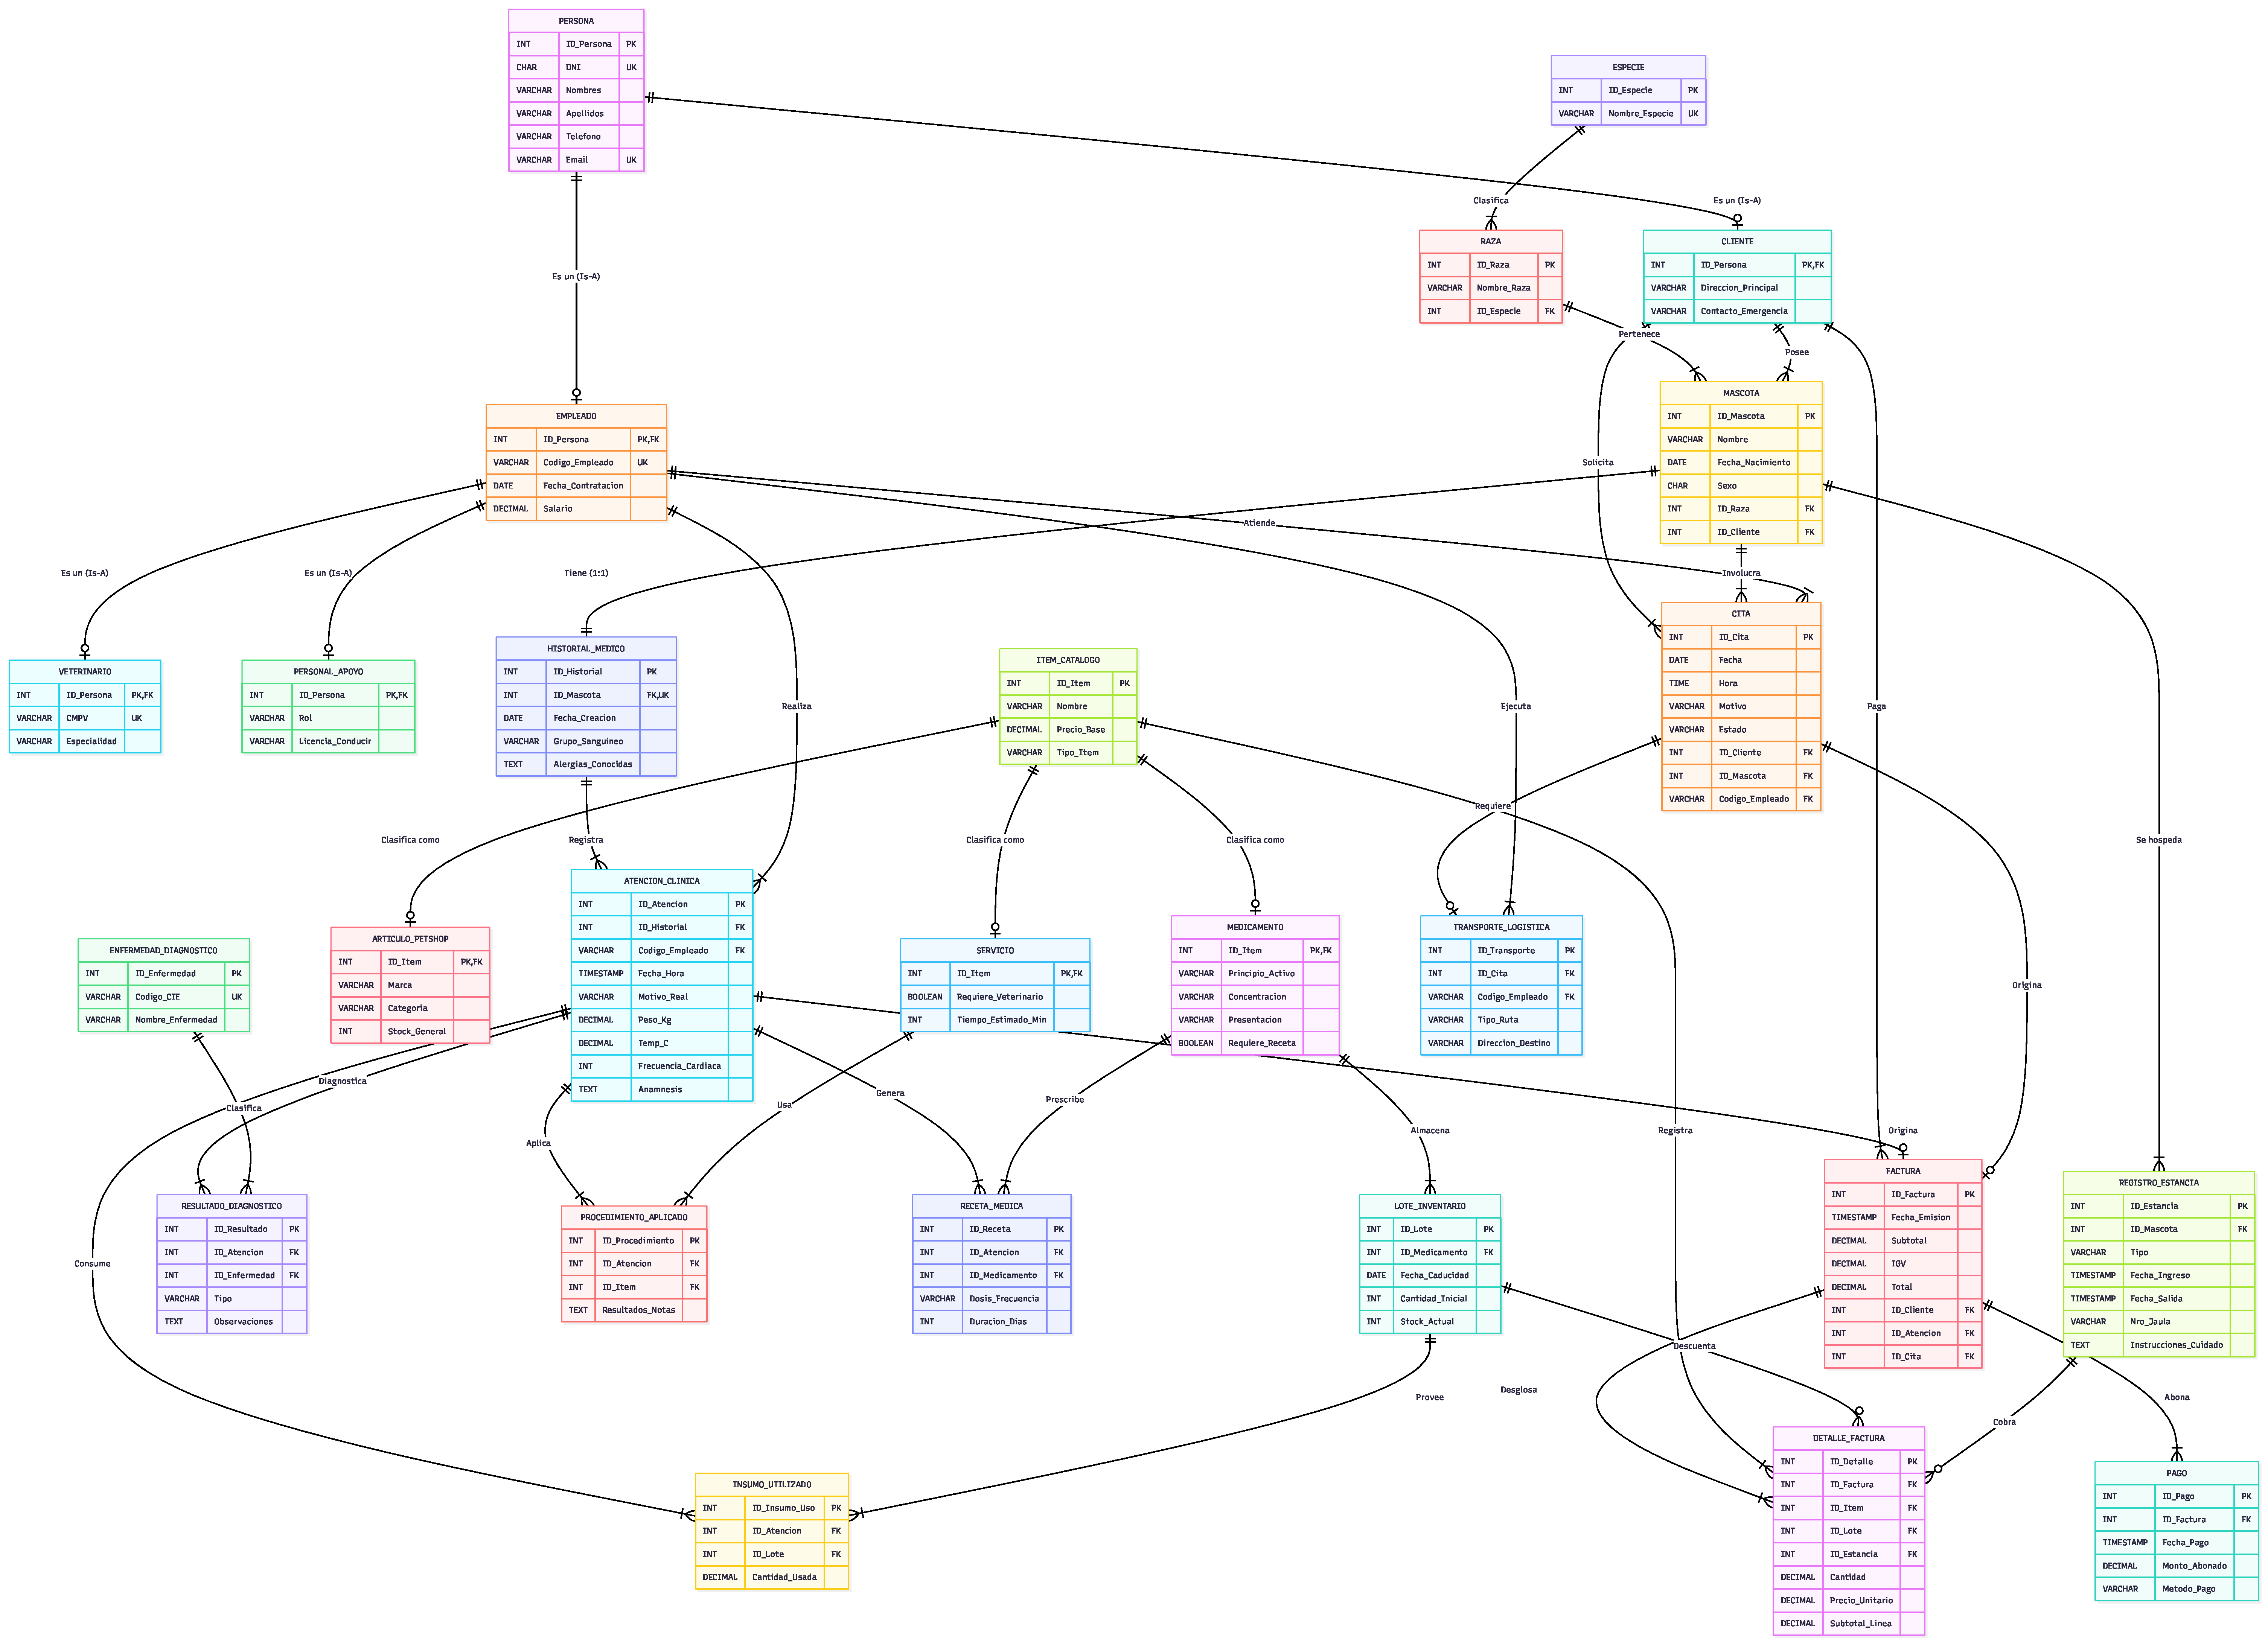
\includegraphics[width=\textwidth]{imagen.pdf}
	\caption{Diagrama Entidad-Relación SOS Veterinaria (Notación Pata de Gallo)}
\end{figure}

\section{Especificaciones y consideraciones del modelo}

A continuación se detalla, entidad por entidad, las especificaciones funcionales y las decisiones de diseño que justifican su estructura dentro del modelo relacional.

\subsection{Persona}

\begin{itemize}
	\item \textbf{Especificaciones:} Almacena los datos personales comunes a todo actor humano del sistema: identificador surrogado (ID\_Persona), documento de identidad (DNI), nombres, apellidos, teléfono de contacto y correo electrónico.
	\item \textbf{Consideraciones:} La llave primaria seleccionada es ID\_Persona, una clave surrogada autoincremenal, en lugar del DNI. Si bien el DNI identifica unívocamente a una persona natural en el Perú, es un dato de negocio sujeto a correcciones administrativas; por ello actúa como clave única alternativa (UK). Esta entidad es una superclase abstracta: ningún registro puede existir en Persona sin pertenecer simultáneamente a Cliente o Empleado. Se implementa el patrón Table Per Subclass (JOINED). Se permite solapamiento: un empleado que también sea cliente tendrá registros en ambas subclases bajo el mismo ID\_Persona.
\end{itemize}

\subsection{Cliente}

\begin{itemize}
	\item \textbf{Especificaciones:} Extiende a Persona con los atributos del titular financiero: Dirección\_Principal y Contacto\_Emergencia. Es la entidad a quien se emiten las facturas y bajo la cual se registran las mascotas.
	\item \textbf{Consideraciones:} Su PK es ID\_Persona (FK $\rightarrow$ Persona), patrón JOINED; no se genera una nueva clave. Dirección\_Principal es NOT NULL porque es requerida para facturación y servicio de transporte. Contacto\_Emergencia es nullable. Un cliente puede poseer múltiples mascotas (relación 1:N con Mascota).
\end{itemize}

\subsection{Empleado}

\begin{itemize}
	\item \textbf{Especificaciones:} Extiende a Persona con los atributos administrativos: Código\_Empleado (UK), Fecha\_Contratación y Salario.
	\item \textbf{Consideraciones:} Su PK es ID\_Persona (FK $\rightarrow$ Persona). Código\_Empleado actúa como clave de negocio alternativa para el sistema de control de acceso. Es a su vez superclase de Veterinario y Personal\_Apoyo bajo el mismo patrón JOINED. El Salario se almacena como referencia administrativa; la liquidación de planillas queda fuera del alcance (véase sección 1.8.2).
\end{itemize}

\subsection{Veterinario}

\begin{itemize}
	\item \textbf{Especificaciones:} Extiende a Empleado con los atributos que validan la habilitación médica: CMPV (número de colegiatura del Colegio Médico Veterinario del Perú, UK) y Especialidad.
	\item \textbf{Consideraciones:} Su PK es ID\_Persona (FK $\rightarrow$ Empleado). El CMPV es la clave única alternativa que otorga validez legal a los actos clínicos (diagnósticos, recetas, cirugías). La regla de integridad que exige que el empleado referenciado en Cita y Atención\_Clínica pertenezca a esta subclase se implementa mediante trigger en la base de datos o validación en la capa de servicio del backend.
\end{itemize}

\subsection{Personal\_Apoyo}

\begin{itemize}
	\item \textbf{Especificaciones:} Extiende a Empleado con el atributo Rol (groomer, chofer, recepcionista) y el campo opcional Licencia\_Conducir.
	\item \textbf{Consideraciones:} Se optó por un atributo discriminador Rol en lugar de crear subclases adicionales (Groomer, Chofer, Recepcionista), ya que estos perfiles no presentan atributos propios que justifiquen tablas separadas. Licencia\_Conducir es nullable y semánticamente válido solo cuando Rol = `Chofer'; esta consistencia se valida en la capa de aplicación.
\end{itemize}

\subsection{Especie}

\begin{itemize}
	\item \textbf{Especificaciones:} Almacena el nivel más alto de clasificación biológica: ID\_Especie (PK surrogada) y Nombre\_Especie (UK, NOT NULL). Ejemplos: Canino, Felino, Exótico, Ave.
	\item \textbf{Consideraciones:} Catálogo de gestión exclusiva del administrador. Nombre\_Especie es UNIQUE para evitar registros duplicados. Su participación en la relación con Raza es parcial: puede existir una especie sin que aún se hayan cargado razas asociadas a ella.
\end{itemize}

\subsection{Raza}

\begin{itemize}
	\item \textbf{Especificaciones:} Almacena la clasificación biológica específica: ID\_Raza (PK surrogada), Nombre\_Raza y ID\_Especie (FK $\rightarrow$ Especie, NOT NULL).
	\item \textbf{Consideraciones:} Si bien el nombre de una raza podría repetirse entre especies distintas (p. ej., ``Mestizo'' para caninos y felinos), se optó por PK surrogada en lugar de llave compuesta (Nombre\_Raza, ID\_Especie), simplificando los JOINS y el mapeo ORM. La FK ID\_Especie es NOT NULL: toda raza debe pertenecer a una especie conocida (participación total).
\end{itemize}

\subsection{Mascota}

\begin{itemize}
	\item \textbf{Especificaciones:} Almacena el perfil del paciente: ID\_Mascota (PK surrogada), Nombre, Fecha\_Nacimiento (nullable), Sexo, ID\_Raza (FK) e ID\_Cliente (FK).
	\item \textbf{Consideraciones:} Fecha\_Nacimiento es nullable porque muchas mascotas rescatadas no tienen fecha de nacimiento conocida. Sexo es NOT NULL dado que es relevante para diagnósticos y procedimientos clínicos. La relación con Cliente es N:1: un cliente puede tener varias mascotas, pero cada mascota pertenece a un único dueño responsable.
\end{itemize}

\subsection{Historial Médico}

\begin{itemize}
	\item \textbf{Especificaciones:} Almacena el expediente clínico permanente: ID\_Historial (PK surrogada), ID\_Mascota (FK, UK), Fecha\_Creación, Grupo\_Sanguíneo (nullable) y Alergias\_Conocidas (nullable).
	\item \textbf{Consideraciones:} Se diseñó como entidad fuerte con PK surrogada en lugar de entidad débil. La regla ``una mascota tiene exactamente un historial'' se garantiza con UNIQUE sobre ID\_Mascota, sin llave compuesta. Esta decisión mejora el rendimiento en JOINs y el mapeo ORM. Los campos de salud son nullable porque se completan progresivamente durante el historial de atenciones.
\end{itemize}

\subsection{Item\_Catálogo}

\begin{itemize}
	\item \textbf{Especificaciones:} Superclase del catálogo de precios. Almacena ID\_Item (PK surrogada), Nombre, Precio\_Base y Tipo\_Item (discriminador de subclase).
	\item \textbf{Consideraciones:} Esta entidad es el corazón de la facturación polimórfica: permite que Detalle\_Factura referencie un único ID\_Item sin importar si es servicio, artículo o medicamento. Tipo\_Item acepta valores controlados: `Servicio', `Articulo', `Medicamento' (CHECK constraint). Se implementa patrón JOINED hacia sus tres subclases.
\end{itemize}

\subsection{Servicio}

\begin{itemize}
	\item \textbf{Especificaciones:} Extiende Item\_Catálogo con Requiere\_Veterinario (boolean, NOT NULL) y Tiempo\_Estimado\_Min (nullable). Representa actividades intangibles: consultas, cirugías, ecografías, baños.
	\item \textbf{Consideraciones:} Requiere\_Veterinario es clave para la validación de citas y procedimientos: si el servicio requiere médico, el empleado asignado debe existir en la tabla Veterinario. Tiempo\_Estimado\_Min es nullable para servicios de duración no predecible (p. ej., cirugías complejas).
\end{itemize}

\subsection{Artículo\_Petshop}

\begin{itemize}
	\item \textbf{Especificaciones:} Extiende Item\_Catálogo con Marca (nullable), Categoría (NOT NULL) y Stock\_General (NOT NULL, DEFAULT 0). Representa bienes físicos de venta libre: alimentos, accesorios, juguetes.
	\item \textbf{Consideraciones:} El stock se gestiona de forma global (un único valor por artículo), a diferencia de los medicamentos que se controlan por lote. Esta simplificación es válida porque los artículos de petshop no tienen fechas de caducidad críticas que requieran trazabilidad por partida. Stock\_General no puede ser negativo (CHECK constraint recomendado).
\end{itemize}

\subsection{Medicamento}

\begin{itemize}
	\item \textbf{Especificaciones:} Extiende Item\_Catálogo con Principio\_Activo, Concentración, Presentación y Requiere\_Receta (boolean). Representa la definición farmacológica genérica, no la existencia física del fármaco.
	\item \textbf{Consideraciones:} La separación entre Medicamento (definición genérica) y Lote\_Inventario (existencia física) es la decisión de diseño más importante del módulo: permite que el veterinario recete el fármaco genérico mientras la farmacia gestiona los lotes físicos de forma independiente. Requiere\_Receta condiciona la dispensación en el módulo de facturación.
\end{itemize}

\subsection{Lote\_Inventario}

\begin{itemize}
	\item \textbf{Especificaciones:} Almacena la existencia física de un medicamento: ID\_Lote (PK surrogada), ID\_Medicamento (FK, NOT NULL), Fecha\_Caducidad, Cantidad\_Inicial y Stock\_Actual.
	\item \textbf{Consideraciones:} Entidad fuerte con PK surrogada. Un mismo medicamento puede tener múltiples lotes activos con distintas fechas de caducidad, habilitando la política FEFO (First Expired, First Out). Stock\_Actual es decrementado tanto por Insumo\_Utilizado (uso clínico) como por Detalle\_Factura (venta en mostrador). Se recomienda un CHECK (Stock\_Actual $>$ 0) y un trigger de alerta cuando el stock caiga por debajo del 15\% de Cantidad\_Inicial.
\end{itemize}

\subsection{Cita}

\begin{itemize}
	\item \textbf{Especificaciones:} Almacena la reserva de tiempo: ID\_Cita (PK), Fecha, Hora, Motivo, Estado, ID\_Cliente (FK), ID\_Mascota (FK) y Código\_Empleado (FK).
	\item \textbf{Consideraciones:} La FK al empleado usa Código\_Empleado (UK de Empleado) para alinearse con el código interno de RRHH. Estado acepta valores controlados: `Pendiente', `Confirmada', `Completada', `Cancelada' (CHECK). Las tres FKs son NOT NULL: una cita requiere los tres actores para ser válida.
\end{itemize}

\subsection{Atención Clínica}

\begin{itemize}
	\item \textbf{Especificaciones:} Registra el acto médico formal: ID\_Atención (PK), ID\_Historial (FK), Código\_Empleado (FK), Fecha\_Hora, Motivo\_Real, Peso\_Kg, Temp\_C, Frecuencia\_Cardíaca y Anamnesis.
	\item \textbf{Consideraciones:} Diseñada como entidad fuerte con PK surrogada para evitar llaves compuestas y facilitar el ORM. Los signos vitales y la anamnesis son nullable porque no toda atención implica una consulta física presencial (algunas son solo revisiones de seguimiento o emisión de recetas). Motivo\_Real puede diferir del Motivo de la Cita que la originó.
\end{itemize}

\subsection{Enfermedad\_Diagnóstico}

\begin{itemize}
	\item \textbf{Especificaciones:} Catálogo de patologías estandarizado según clasificación CIE: ID\_Enfermedad (PK), Código\_CIE (UK) y Nombre\_Enfermedad (NOT NULL).
	\item \textbf{Consideraciones:} El Código\_CIE garantiza uniformidad en la nomenclatura médica, evitando variaciones textuales del mismo diagnóstico (p. ej., ``Parvovirus'' vs. ``Parvo'' vs. ``Parvovirosis''). Es un catálogo de solo lectura para los veterinarios; su mantenimiento es responsabilidad exclusiva del administrador. Esta estandarización habilita las consultas epidemiológicas (Q1) de la sección 1.5.4.
\end{itemize}

\subsection{Resultado\_Diagnóstico}

\begin{itemize}
	\item \textbf{Especificaciones:} Vincula una atención con una enfermedad diagnosticada: ID\_Resultado (PK), ID\_Atención (FK), ID\_Enfermedad (FK), Tipo y Observaciones (nullable).
	\item \textbf{Consideraciones:} Entidad transaccional fuerte que permite múltiples diagnósticos por atención (1:N desde Atención\_Clínica). Tipo solo acepta `Presuntivo' o `Definitivo' (CHECK constraint), diferenciando una sospecha clínica de un diagnóstico confirmado. La participación es total: todo resultado debe estar vinculado a una atención y a una enfermedad del catálogo.
\end{itemize}

\subsection{Procedimiento\_Aplicado}

\begin{itemize}
	\item \textbf{Especificaciones:} Registra las intervenciones médicas ejecutadas: ID\_Procedimiento (PK), ID\_Atención (FK), ID\_Item (FK $\rightarrow$ Servicio) y Resultados\_Notas (nullable).
	\item \textbf{Consideraciones:} La FK ID\_Item referencia específicamente la subclase Servicio dentro de Item\_Catálogo, garantizando que solo se registren como procedimientos ítems de tipo servicio, nunca artículos ni medicamentos. Permite múltiples procedimientos por atención. Resultados\_Notas es nullable para procedimientos rutinarios sin hallazgos adicionales.
\end{itemize}

\subsection{Insumo Utilizado}

\begin{itemize}
	\item \textbf{Especificaciones:} Descarga de inventario clínico: ID\_Insumo\_Uso (PK), ID\_Atención (FK), ID\_Lote (FK) y Cantidad\_Usada.
	\item \textbf{Consideraciones:} Es el mecanismo que cierra el ciclo de inventario durante el acto médico: al registrar un insumo, el sistema debe decrementar Stock\_Actual del Lote\_Inventario correspondiente (trigger o lógica de servicio). Cantidad\_Usada debe ser $>$ 0 (CHECK) y no puede superar el stock disponible. A diferencia de Receta\_Médica, referencia el lote específico, no el medicamento genérico.
\end{itemize}

\subsection{Receta Médica}

\begin{itemize}
	\item \textbf{Especificaciones:} Prescripción farmacológica del veterinario: ID\_Receta (PK), ID\_Atención (FK), ID\_Medicamento (FK), Dosis\_Frecuencia y Duración\_Días.
	\item \textbf{Consideraciones:} Referencia Medicamento (genérico) y no Lote\_Inventario, porque la receta es un acto médico, no una transacción de stock. El descuento de inventario ocurre cuando el dueño adquiere el medicamento en la farmacia, registrado en Detalle\_Factura vinculado al lote específico. Esta separación de responsabilidades es intencional y refleja el flujo real de la clínica.
\end{itemize}

\subsection{Registro\_Estancia}

\begin{itemize}
	\item \textbf{Especificaciones:} Controla la ocupación de hospedaje e internamiento: ID\_Estancia (PK), ID\_Mascota (FK), Tipo, Fecha\_Ingreso, Fecha\_Salida (nullable), Nro\_Jaula (NOT NULL) e Instrucciones\_Cuidado (nullable).
	\item \textbf{Consideraciones:} Tipo acepta `Guardería' o `Internamiento' (CHECK), diferenciando una estadía vacacional de una post-operatoria. Fecha\_Salida es nullable porque la mascota puede seguir hospitalizada al momento de la consulta. El cobro de la estancia se realiza en Detalle\_Factura mediante la FK opcional ID\_Estancia, cerrando el ciclo de facturación de hospedajes.
\end{itemize}

\subsection{Transporte\_Logística}

\begin{itemize}
	\item \textbf{Especificaciones:} Gestiona el servicio de taxi veterinario: ID\_Transporte (PK), ID\_Cita (FK), Código\_Empleado (FK), Tipo\_Ruta, Dirección\_Destino, Estado.
	\item \textbf{Consideraciones:} La relación con Cita es 1:1: una cita puede generar como máximo un registro de transporte. Tipo\_Ruta acepta `Recojo' o `Entrega' (CHECK). La regla de que el empleado asignado debe tener Rol = `Chofer' en Personal\_Apoyo se implementa mediante trigger o validación en la capa de servicio.
\end{itemize}

\subsection{Factura}

\begin{itemize}
	\item \textbf{Especificaciones:} Comprobante legal de la transacción: ID\_Factura (PK), Fecha\_Emisión, Subtotal, IGV, Total, ID\_Cliente (FK), ID\_Atención (FK, nullable) e ID\_Cita (FK, nullable).
	\item \textbf{Consideraciones:} Las FK ID\_Atención e ID\_Cita son mutuamente excluyentes, reguladas mediante CHECK constraint: no pueden ser ambas NOT NULL simultáneamente. Si ambas son NULL, la factura corresponde a una compra libre en el mostrador de petshop. Esta restricción garantiza la trazabilidad del origen de cada cobro sin duplicar tablas de facturación.
\end{itemize}

\subsection{Detalle Factura}

\begin{itemize}
	\item \textbf{Especificaciones:} Desglose de ítems cobrados: ID\_Detalle (PK), ID\_Factura (FK), ID\_Item (FK), ID\_Lote (FK, nullable), ID\_Estancia (FK, nullable), Cantidad, Precio\_Unitario y Subtotal\_Línea.
	\item \textbf{Consideraciones:} Esta entidad tiene función dual: es el desglose financiero de la factura y el mecanismo que cierra el ciclo de inventario al vender un medicamento (vinculando el lote específico vía ID\_Lote). Regla semántica: si ID\_Item es un Medicamento, ID\_Lote no puede ser NULL; si corresponde a hospedaje, ID\_Estancia no puede ser NULL. Estas restricciones condicionales se implementan en la capa de servicio.
\end{itemize}

\subsection{Pago}

\begin{itemize}
	\item \textbf{Especificaciones:} Registra cada ingreso monetario: ID\_Pago (PK), ID\_Factura (FK), Fecha\_Pago, Monto\_Abonado y Método\_Pago.
	\item \textbf{Consideraciones:} La relación 1:N con Factura habilita los pagos fraccionados: una factura puede abonarse en múltiples cuotas o con distintos medios en un mismo acto (p. ej., parte en efectivo y parte en Yape). Método\_Pago acepta valores controlados: `Efectivo', `Tarjeta Débito', `Tarjeta Crédito', `Yape', `Plin' (CHECK constraint). La validación de que la suma de abonos no supere el total de la factura se implementa en la capa de servicio.
\end{itemize}
